% Simple example figure generated with TikZ
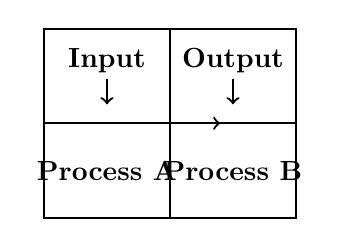
\begin{tikzpicture}[scale=0.8]
    % Draw a simple diagram
    \draw[thick] (0,0) rectangle (4,3);
    \draw[thick] (2,0) -- (2,3);
    \draw[thick] (0,1.5) -- (4,1.5);

    % Add some text
    \node at (1,2.5) {\textbf{Input}};
    \node at (3,2.5) {\textbf{Output}};
    \node at (1,0.75) {\textbf{Process A}};
    \node at (3,0.75) {\textbf{Process B}};

    % Add arrows
    \draw[->, thick] (1,2.2) -- (1,1.8);
    \draw[->, thick] (3,2.2) -- (3,1.8);
    \draw[->, thick] (2.2,1.5) -- (2.8,1.5);
\end{tikzpicture}